\chapter{Spezifikation der funktionellen Anforderungen}
\section{Produktbeschreibung}
TODO: Blablabla, alles wichtig und ganz toll

\section{Funktionelle Anforderungen}
\subsection{Umgebungsmodell}

\subsubsection{Ereignistabelle}
%wenn die Tabellen zu lang werden -> longtable
TODO:
\begin{tabular}[ht]{|l|l|l|l|}
\hline
Nr & Ereignis & Datenfluß im System & Antwort des Systems \\
\hline\hline
1. & A ändert oder Ergänzt Bucherliste & Bücherdaten & Bestätigung\_Bücheränderung \\
2. & B macht auch was & Zahlungen & Ignorieren\_Änderungen \\
2. & B macht auch was & Zahlungen & Ignorieren\_Änderungen \\
2. & B macht auch was & Zahlungen & Ignorieren\_Änderungen \\
\hline
\end{tabular}

\subsubsection{Kontextdiagramm}
TODO
%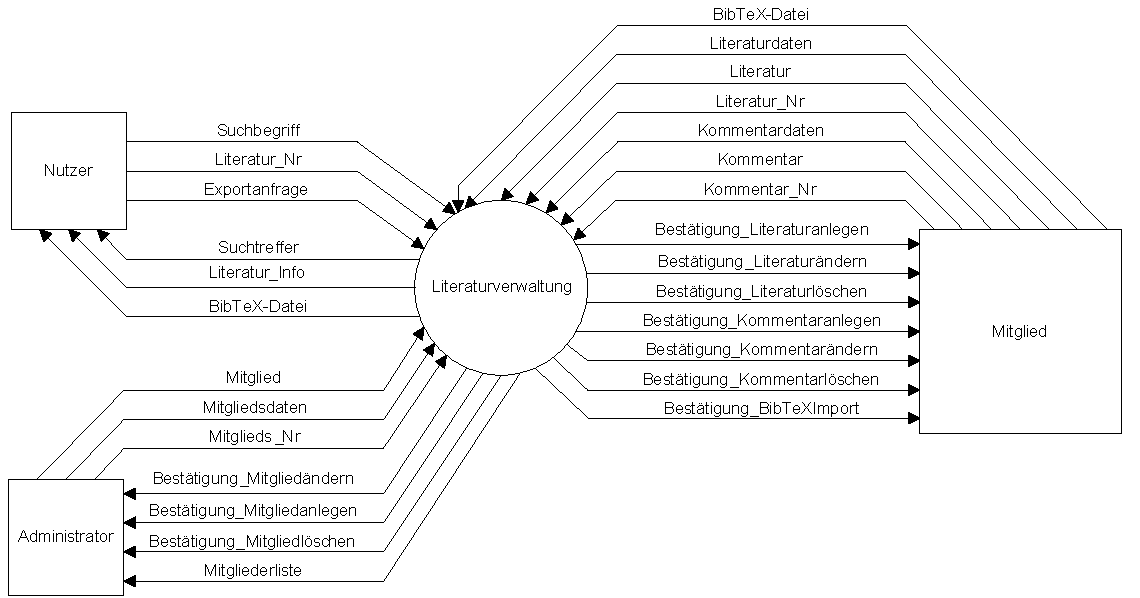
\includegraphics[scale=0.5]{kontextdiagramm}
% oder \centerline{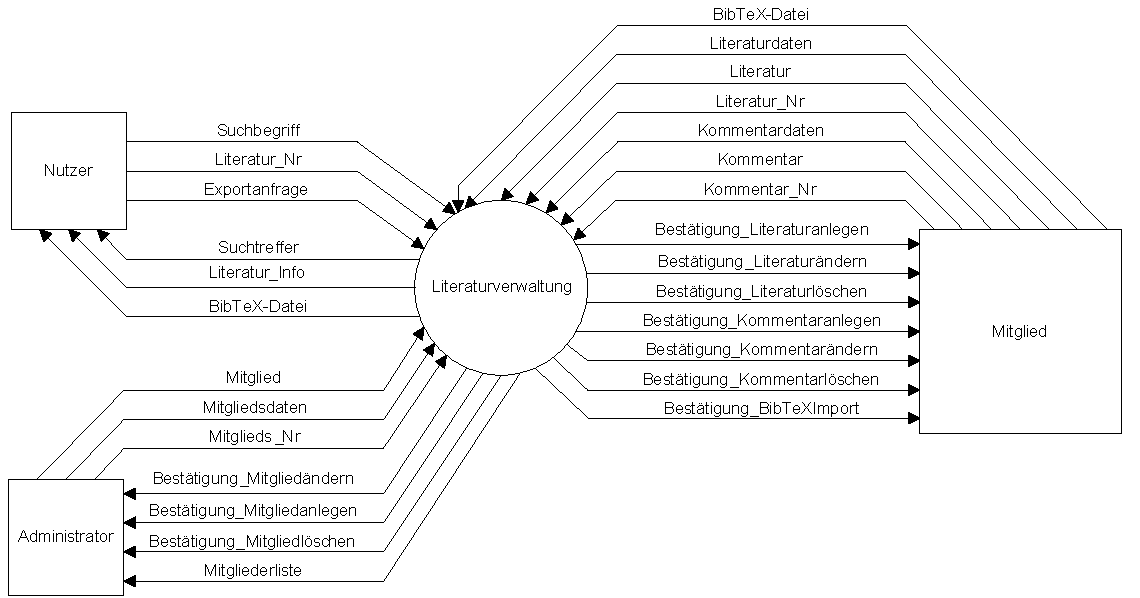
\includegraphics[scale=0.5]{kontextdiagramm}}

\subsection{Verhaltensmodell}
\subsubsection{Grobes Verhaltensmodell (vergröbertes primäres Verhaltensmodell)}
TODO
%\includegraphics[scale=0.5]{verhaltensmodell_grob}

\subsubsection{Primäres Verhaltensmodell}
\paragraph{Teilmodell blabla}
TODO
%\includegraphics[scale=0.5]{erhaltensmodell_blabla}

\paragraph{Teilmodell bloblo}
TODO
%\includegraphics[scale=0.5]{verhaltensmodell_bloblo}

\subsubsection{Verfeinerungen der Prozesse des primären Verhaltensmodells}
\paragraph{Verfeinerung zum Prozess: ieeekks}
TODO
%\includegraphics[scale=0.5]{prozess_ieeekks}

\paragraph{Verfeinerung zum Prozess: arrgghhh}
TODO
%\includegraphics[scale=0.5]{prozess_arrgghhh}

\subsubsection{Datenkatalog}
TODO:
\begin{tabular}[ht]{|l|l|}
\hline
Element & Strukturbeschreibung \\
\hline\hline
% Mitglieder
\emph{Mitglieder} & \{Mitglied\} \\
Mitglied  & M\_Name + Anschrift + <Beitritts>Datum + @Parzellen\_Nr + (Funktion) \\
\hline\hline
\emph{Leistungen} & {Leistung} \\
.... & ... \\
\hline
\end{tabular}

\subsubsection{Beziehungen zwischen Speichern (ERD)}
%wenn die Tabellen zu lang werden -> longtable
TODO:
%\includegraphics[scale=0.5]{erd}

\subsubsection{Prozessspezifikation}
TODO: (siehe Beispielbeleg S. 9)

\paragraph{Prozess abc}

\paragraph{Prozess cde}

\subsection{Definition der Nutzerschnittstelle}
TODO (Generell, Fargestaltung)

\subsubsection{Ein- und Ausgabegeräte}
TODO Siehe Beispielbeleg S. 11

\paragraph{Legende zur Layoutdarstellung}
TODO Siehe Beispielbeleg S. 11

\paragraph{Grundfenster}
TODO

\paragraph{Menüs}
TODO

\paragraph{Fenster irgendwas}
TODO